
\begin{figure}[tbh]
  \begin{center}
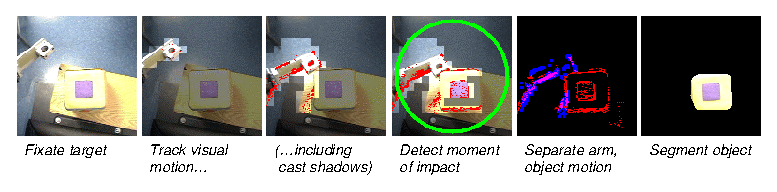
\includegraphics[width=\columnwidth]{fig-poke-zoom.eps}
%%    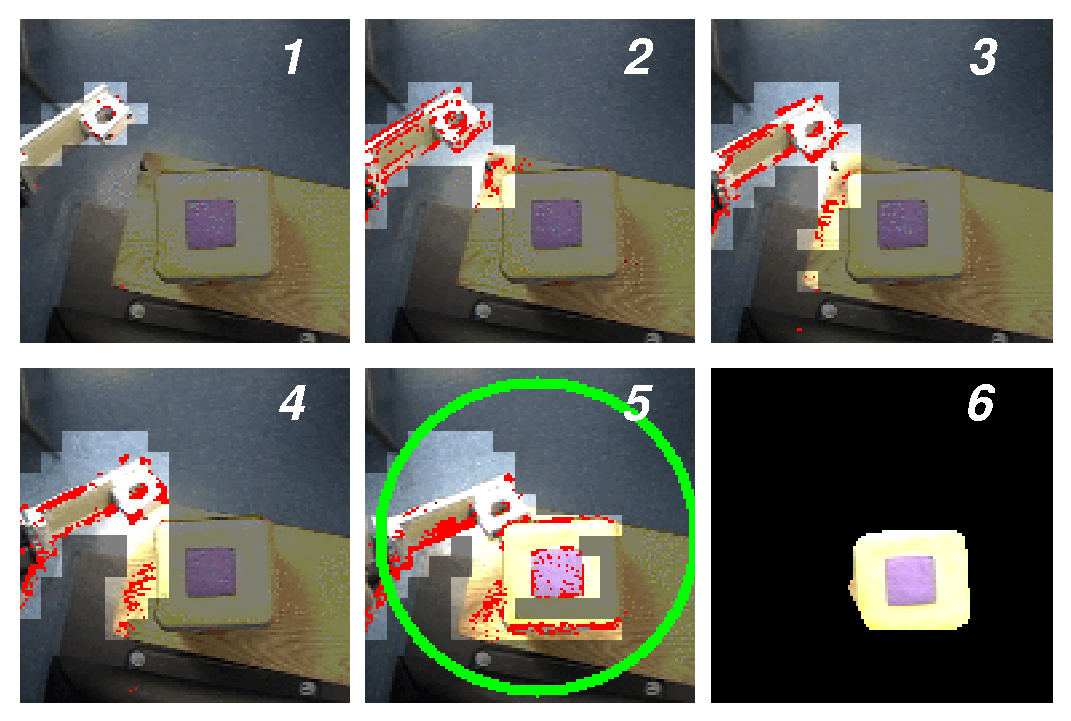
\includegraphics[width=8cm]{collision-detail}
  \end{center}
  \caption{
  \label{fig:poke-zoom}
    The moment of impact is detected visually by the
    sudden expansion of motion away from the arm.  Motion before and
    after contact is compared to gather information for segmentation.
}
\end{figure}


\subsubsection*{The moment of (ground) truth}

How can we detect when the arm collides with an object?  One natural
possibility would be to use proprioceptive or tactile information from
the arm itself.  Another possibility is to detect the collision
visually.  This is the method we use since, as
Section~\ref{sect:manipulator} will discuss, it allows collision
detection to be applied to human arm motion, a situation where the robot
does not have access to any privileged information about the motion.  When the robot 
is attempting to poke a target, it keeps the target fixated,
so that the image processing does not need to compensate for
egomotion.
Under these conditions, it is possible to detect motion using
image differencing.
This is a very simple technique for detecting motion by
simply subtracting successive frames coming from a camera and looking for
pixel-level differences.  A moving object that has some contrast with
the background it is moving over will generate such differences.  Of
course, pixel differences can also be generated by changes in
illumination, cast shadows, the refresh rate of computer monitors, movement of the camera
itself, etc.  A related technique called background modeling tries to
estimate the appearance of the fixed, stationary background of a 
scene, and then subtract the current view from the reference to 
detect new foreground.  Cog uses such a technique to detect motion
while it is fixating a target.

%% While these techniques are not ideally
%% suited to a moving platform like our robot, they are short periods 
%% during which they can be useful.  In particular, when the robot is
%% fixating a target, we can do this.

%%Two components -- detecting the moment of impact, and extracting as 
%%much data as possible from the frames around it.

%%There are particular periods when the robot is attentive and fixating.
%%When this is so, it can detect visually when a collision occurs
%%between a moving object and a previously stationary object in view.
%%The principal task, then, is keep the motion of the moving object distinct
%%from that of the impacted object.

%%Brief introduction to image differencing and background subtraction.
%%Stationary camera assumption to facilitate pixel modeling.  Don't want
%%to keep head stationary, but can fixate for significant periods.

Figure~\ref{fig:poke-zoom} shows the sequence of processing steps
taken as the arm approaches and comes into contact with a target.  As
the arm approaches, its motion is tracked very coarsely in real-time,
and areas it passes through are marked as ``clear'' of the object.  An impact event
is detected through a signature explosion of movement connected with
the arm, but spread across a much wider distance than the arm could
possibly have moved in the time available.  Once this impact is detected, we
start to process at high resolution (and drop briefly out of real-time
operation for a few seconds).  The raw motion signature generated by
the collision is computed.  The translational component of the arm
motion at the point of contact is also computed, so that motion present in
previous frames can be aligned with the collision frame, and motion 
associated with the arm can be isolated from motion
due to the target object.  Since the impact may occur just before a
frame is sampled (every 30 milliseconds) and so generate a relatively
weak motion signature, motion information from one frame after
collision is projected back and pooled with motion information in the
collision frame.  In the absence of strong texture there may be little apparent motion
 in the interior of the object, so we recruit a maximum-flow
algorithm due to \cite{boykov01experimental} to fill in such regions
efficiently.
%
Figure~\ref{fig:poking-segmentation} shows examples of segmentations
generated by very different poking operations -- one a gentle
tap from the side, the other a violent ``back-slap'' striking
the object away from the robot.

%%Within the context of the robot fixating a target, we try to detect
%%the moment of impact precisely, so we can apply the (relatively) slow
%%segmentation optimization to a narrow interval of the video input and
%%maintain close to real-time performance.  A moving manipulator
%%colliding with an object will accelerate it, if it is not too massive.
%%If the object is rigid, the motion of the manipulator will be transmitted 
%%through it.  This transmission can be detected as a spreading motion
%%that is not plausibly generated by the manipulator itself.

%%Some assumptions that may fail: object not too heavy; object at least
%%semi-rigid; manipulator not moving above a certain speed; manipulator
%%not casting shadows on the object itself.  When the robot is poking the
%%object itself, it can control some of this.  If the object iself is
%%troublesome, then we potentially diagnose this, or just ignore it.

%%We are relying on some facts about optic flow.  When an object is ...


%
\begin{figure}[tb]
\begin{center}
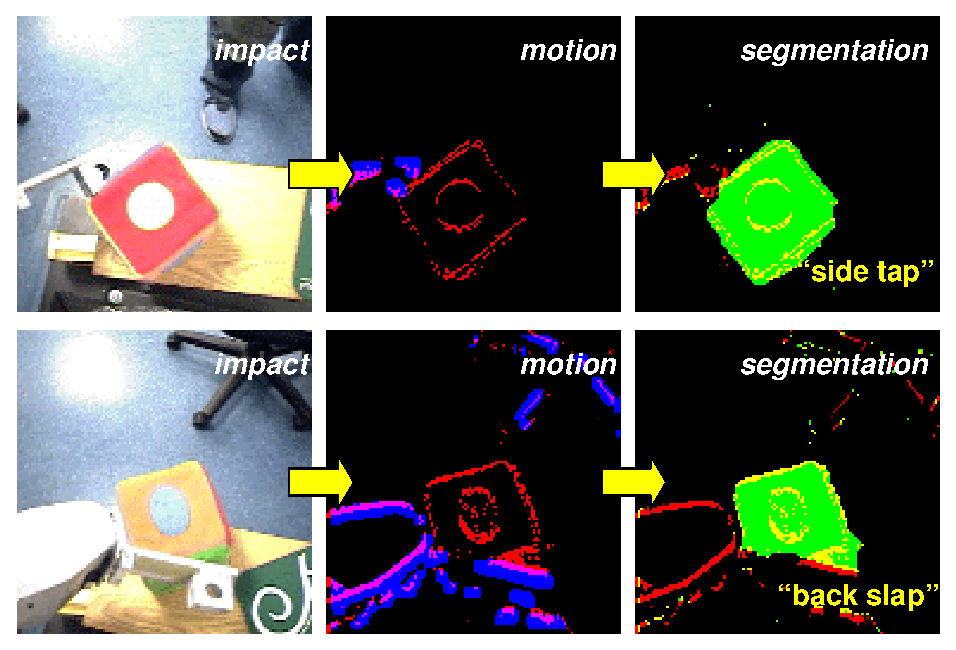
\includegraphics[width=10cm]{fig-poke-batting.eps}
%%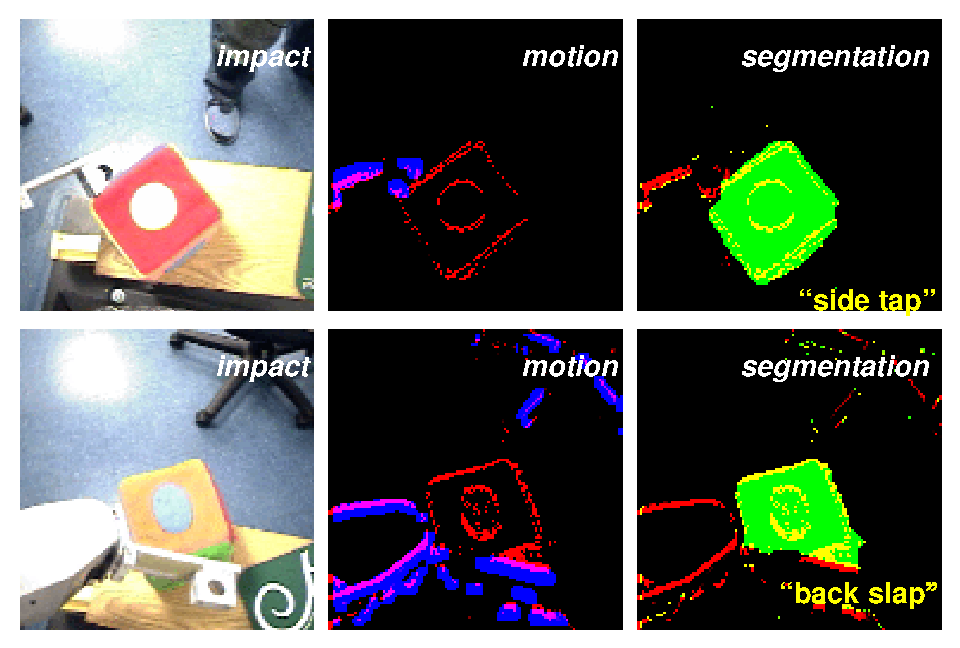
\includegraphics[width=8cm]{segmentation-detail.eps}
%%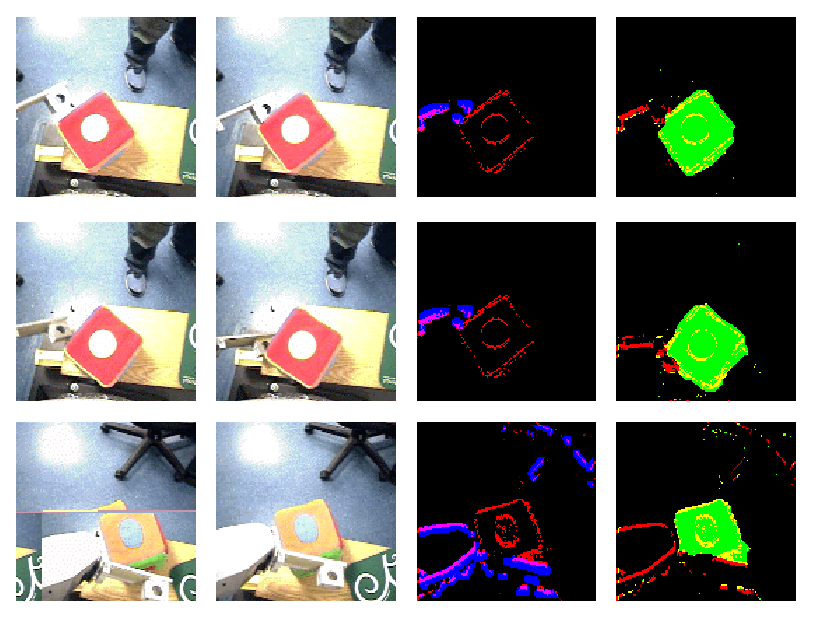
\includegraphics[width=\columnwidth]{poking_segmentation.eps}
\caption{ 
\label{fig:poking-segmentation}
%
Cog batting a cube around.  The top row shows the flipper poking
an object from the side, turning it slightly.  The second
row shows Cog batting an object away.  The images in the first column
are frames prior to a collision.  The second column shows the actual
impact.  The third column shows the motion signal at the point of
contact.  The bright regions in the images in the final column show
the segmentations produced for the object. 
%
}
\end{center}
\end{figure}
%


